\documentclass{article}

\usepackage{amsmath, amsfonts, microtype, xcolor, tikz, graphicx}
\usepackage[hidelinks]{hyperref}
\usepackage[]{neurips_2019}
\DeclareMathOperator{\Tr}{Tr}

\usetikzlibrary{calc}

\tikzset{
    ncbar angle/.initial=90,
    ncbar/.style={
        to path=(\tikztostart)
        -- ($(\tikztostart)!#1!\pgfkeysvalueof{/tikz/ncbar angle}:(\tikztotarget)$)
        -- ($(\tikztotarget)!($(\tikztostart)!#1!\pgfkeysvalueof{/tikz/ncbar angle}:(\tikztotarget)$)!\pgfkeysvalueof{/tikz/ncbar angle}:(\tikztostart)$)
        -- (\tikztotarget)
    },
    ncbar/.default=0.5cm,
}

\tikzset{round left paren/.style={ncbar=0.5cm,out=110,in=-110}}
\tikzset{round right paren/.style={ncbar=0.5cm,out=70,in=-70}}

\newcommand{\dlp}[1]{{\color{red} (DLP: #1)}}
\newcommand{\mo}[1]{{\color{green} (MO: #1)}}
\newcommand{\jrk}[1]{{\color{blue} (JRK: #1)}}
\newcommand{\fc}[1]{{\color{orange} (FC: #1)}}

\title{Discovering causal factors with back-and-forth regression}

\author{%
  Jean-Remi King\\
  CNRS\\
  \texttt{email} \\
  \And
  Fran\c{c}ois Charton\\
  Facebook AI\\
  \texttt{fcharton@fb.com}\\
  \And
  David Lopez-Paz\\
  Facebook AI\\
  \texttt{dlp@fb.com}
  \And
  Maxime Oquab\\
  Facebook AI\\
  \texttt{qas@fb.com}
}

\begin{document}

\maketitle

\begin{abstract}
Identifying causes from observations is at the core of science. This endeavor
is particularly challenging when i) potential factors are difficult to
manipulate individually and ii) observations are complex and multi-dimensional.
To address this issue, we introduce ``back-and-forth regression'' (BFR), a
method designed to identify, from a set of co-varying factors, the factors
that most plausibley account for multidimensional observations. After detailing
the proof of convergence, we show that BFR outperforms least-squares and related
regression techniques, as well as cross-decomposition methods (e.g. canonical
correlation analysis, and partial least squares) on two tasks: causal
identification and out-of-distribution prediction. Finally, we apply BFR to
neuroimaging recordings of 102 subjects reading word sequences. The results
show, as expected, that the early brain responses to words appear to be
specifically caused by low-level visual factors whereas late brain responses
appear to be caused by lexical factors, despite the fact that these factors
covary in the study.
% conclude  open
\end{abstract}

\section{Introduction}

Natural sciences are tasked to find, from a set of hypothetical factors, the minimal subset that suffices to reliably predict novel observations potentially in novel environments.
%
This problem can be formalized as follow: empirical studies consist in measuring, via an apparatus $F$, a signal $Y \in \mathbb{R}^{i, l}$, that is a function of possible causes $X \in \mathbb{R}^{i, j}$, and other unknown causes that can be understood as noise $N \in \mathbb{R}^{i, k}$: $Y=F(X,N)$. Of all considered causes (features of X), only a subset accounts for $Y$, let it be represented as $E \cdot X$, with $E \in \mathbb{R}^{j, j}$ a binary diagonal matrix, which selects causal features of $X$.
%
Under the restricted assumptions of centered and additive noise N and linear systems, causal discovery thus consists in finding $E$ in

\begin{equation}
    Y=(XEM+N)F
\end{equation}
with $M \in \mathbb{R}^{j, k}$ and $F \in \mathbb{R}^{j, k}$ being unknown.  $M$ is a unknown projection matrix that ensures that the noise and the causal factors share a common space, and can thus be absorbed by $F$:
\begin{equation}
    Y=(XE+N^{*})F^{*}
\end{equation}
\par

%
Under this formalism, causal discovery is impeded by two challenges.
%
To illustrate these two challenges, let us consider the case of a neuroscientist who studies the brain bases of reading. Our neuroscientist wants to determine whether the frequency of a word modulates brain activity (e.g. neurons may become more active when our retina is flashed with the word 'triskaidekaphobia' than when the word is 'car'). One issue is that word frequency tends to correlate with word length.\par
%
%
This is the first challenge to causal discovery: a set of putative factors, some causal, other non-causal, can be collinear. Collinearity in the putative factors $X$ is typically addressed with factorial designs \cite{fisher_1935}. For example, our neuroscientist may carefully select words matched in terms of length, while letting their frequency vary. However, factorial design becomes increasingly difficult to implement as the number of considered factor grows. As a fallback option, factors may be orthogonalized \textit{a posteriori}, by analytically estimating how each of them contributes to explaining the observations. Our neuroscientist will thus typically use ordinary least square (OLS) to model how brain activity can be specifically accounted for by word length and word frequency:
\begin{equation}
H = (X'X)^{-1} X'Y
\end{equation}
In this paper, we refer to this approach as 'forward modeling' as it models how the factors X contribute to explain the observations Y. \par
%
%
The second challenge to causal discovery is the multiplicity of the observations. For example, our neuroscientist may simultaneously collect noisy recordings of hundreds of thousands of neurons. It can thus be suboptimal to consider each neuron independently, because they may be influenced by some unknown factors $N$. More generally, with the rise of large and complex datasets, the complexity of observations has led many to invert the problem and to focus on optimally predicting putative factors from complex and poorly controlled observations. In neuroimaging, for example, it is increasingly popular to use "decoding" methods: instead of testing whether the brain responds to particular factors, a model is trained to maximally predict factors from complex brain signals:
\begin{equation}
G = (Y'Y)^{-1} Y'X
\end{equation}
We refer to this approach as 'backward modeling' as it models how the observations Y can be combined to predict the factors X. \par
%
%
As illustrated in Fig. 1., both forward and backward modeling have competing benefits and drawbacks. Specifically, forward modeling efficiently disentangles the independent contribution of collinear factors, but does not combine multidimensional observations. By contrast, backward modeling combines multiple observations, but does not disentangle collinear factors. \par
%
%
In this paper, we introduce the 'back-and-forth regression', which combines the benefits of forward and backward modeling. Back-and-forth regression consists in first predicting X from Y (as in the backward modeling) subsequently retrieving an estimate $\hat X$ and finally disentangling which of the considered factors X accounts for the variance in $\hat X$ (i.e. analogously to forward modeling). \par
%
In the next sections, we detail back-and-forth regression, prove that it asymptotically extracts E, and show how it relates to and departs from other cross-decomposition and component analyses. We then show with synthetic experiments that back-and-forth regression outperforms state-of-the-art techniques for regression and feature extraction, both in terms of causal discovery and out-of-environment predictions. Finally, we apply back-and-forth regression to the brain activity of 102 subjects reading $\approx$ 2,000 words, and show that the first brain responses to these words appear to be mainly modulated by low-level visual features, such as the number of letters, while late brain responses appear to be mainly modulated by high-level lexical features, such as word frequency. \par
%

\section{Back an forth regression}

\begin{figure}[t!]
    \centering
    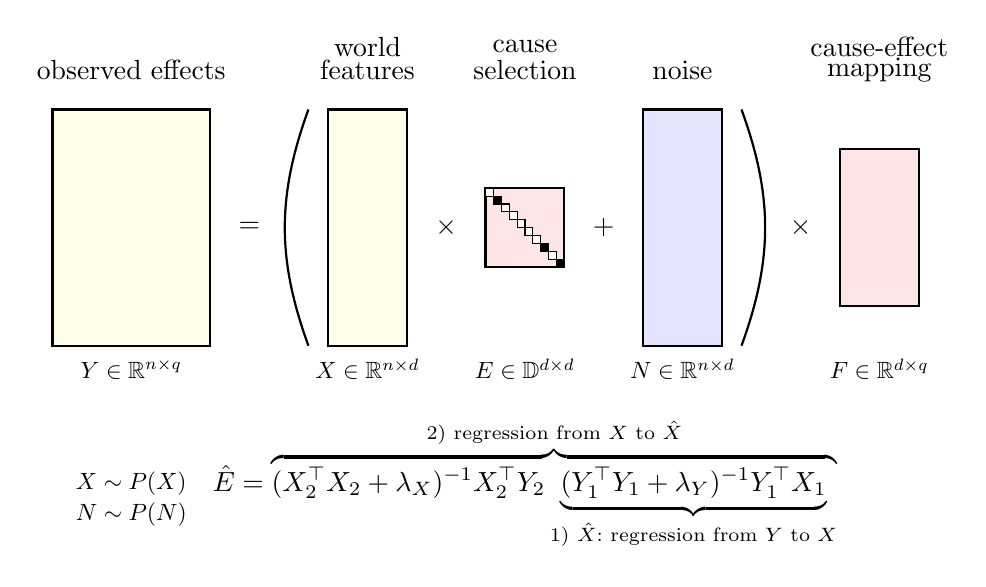
\begin{tikzpicture}
    \newcommand\posY{0}
    \newcommand\posX{3}
    \newcommand\posE{5}
    \newcommand\posN{7}
    \newcommand\posF{9.5}

    \node[thick, draw=black, minimum height=3cm, minimum width=2cm, fill=yellow!10] (Y) at (\posY, 0){};
    \node[] (eq) at (1.5, 0){$=$};
    \node[] (times) at (4, 0){$\times$};
    \node[thick, draw=black, minimum height=3cm, minimum width=1cm, fill=yellow!10] (X) at (\posX, 0){};
    \node[thick, draw=black, minimum height=1cm, minimum width=1cm, fill=red!10] (E) at (\posE, 0){};

    \draw[fill=white] (\posE - 0.5 + 0.0, 0.5 - 0.0) rectangle (\posE - 0.5 + 0.0 + 0.1, 0.5 - 0.0 - 0.1);
    \draw[fill=black] (\posE - 0.5 + 0.1, 0.5 - 0.1) rectangle (\posE - 0.5 + 0.1 + 0.1, 0.5 - 0.1 - 0.1);
    \draw[fill=white] (\posE - 0.5 + 0.2, 0.5 - 0.2) rectangle (\posE - 0.5 + 0.2 + 0.1, 0.5 - 0.2 - 0.1);
    \draw[fill=white] (\posE - 0.5 + 0.3, 0.5 - 0.3) rectangle (\posE - 0.5 + 0.3 + 0.1, 0.5 - 0.3 - 0.1);
    \draw[fill=white] (\posE - 0.5 + 0.4, 0.5 - 0.4) rectangle (\posE - 0.5 + 0.4 + 0.1, 0.5 - 0.4 - 0.1);
    \draw[fill=white] (\posE - 0.5 + 0.5, 0.5 - 0.5) rectangle (\posE - 0.5 + 0.5 + 0.1, 0.5 - 0.5 - 0.1);
    \draw[fill=white] (\posE - 0.5 + 0.6, 0.5 - 0.6) rectangle (\posE - 0.5 + 0.6 + 0.1, 0.5 - 0.6 - 0.1);
    \draw[fill=black] (\posE - 0.5 + 0.7, 0.5 - 0.7) rectangle (\posE - 0.5 + 0.7 + 0.1, 0.5 - 0.7 - 0.1);
    \draw[fill=white] (\posE - 0.5 + 0.8, 0.5 - 0.8) rectangle (\posE - 0.5 + 0.8 + 0.1, 0.5 - 0.8 - 0.1);
    \draw[fill=black] (\posE - 0.5 + 0.9, 0.5 - 0.9) rectangle (\posE - 0.5 + 0.9 + 0.1, 0.5 - 0.9 - 0.1);

    \node[] (plus) at (6, 0){$+$};
    \node[thick, draw=black, minimum height=3cm, minimum width=1cm, fill=blue!10] (N) at (\posN, 0){};
    \node[thick, draw=black, minimum height=2cm, minimum width=1cm, fill=red!10] (F) at (\posF, 0){};
    \draw [thick] (2.25, -1.5) to [round left paren ] (2.25, 1.5);
    \draw [thick] (7.75, -1.5) to [round right paren ] (7.75, 1.5);

    \node[] (times2) at (8.5, 0){$\times$};

    \node[] (annY) at (\posY, -1.8){\scalebox{0.85}{$Y \in \mathbb{R}^{n \times q}$}};
    \node[] (annX) at (\posX, -1.8){\scalebox{0.85}{$X \in \mathbb{R}^{n \times d}$}};
    \node[] (annE) at (\posE, -1.8){\scalebox{0.85}{$E \in \mathbb{D}^{d \times d}$}};
    \node[] (annN) at (\posN, -1.8){\scalebox{0.85}{$N \in \mathbb{R}^{n \times d}$}};
    \node[] (annF) at (\posF, -1.8){\scalebox{0.85}{$F \in \mathbb{R}^{d \times q}$}};

    \node[] (labY) at (\posY, 2){observed effects};
    \node[] (labX) at (\posX, 2.3){world};
    \node[] (labX) at (\posX, 2){features};
    \node[] (labE) at (\posE, 2.3){cause};
    \node[] (labE) at (\posE, 2){selection};
    \node[] (labN) at (\posN, 2){noise};
    \node[] (labF) at (\posF, 2.3){cause-effect};
    \node[] (labF) at (\posF, 2){mapping};

    \node[] (sim1) at (0,-3.25) {\scalebox{0.85}{$X \sim P(X)$}};
    \node[] (sim2) at (0,-3.65) {\scalebox{0.85}{$N \sim P(N)$}};
    \node[] (reg1) at (5,-3.25) {$\hat{E} = \overbrace{(X_2^\top X_2 + \lambda_X)^{-1} X_2^\top Y_2\underbrace{(Y_1^\top Y_1 + \lambda_Y)^{-1} Y_1^\top X_1}_{\text{1) } \hat{X} : \text{ regression from } Y \text{ to } X}}^{\text{2) regression from } X \text{ to } \hat{X}} $};
    \end{tikzpicture}
    \caption{Summary of our method blah blah blah}
    \label{fig:}
\end{figure}


\subsection{Algorithm}

Back and forth regression consists in two steps.
%
First, we perform a least squares estimation of X from Y, that is we find $\hat G$ such that $\hat X=\hat G Y$ is the least square predictor of X.
%
This recovers an approximation of the causes of Y in X.
%
Then, we perform a least squares estimation of $\hat X$ from X, and determine $\hat H$ such that $\hat {\hat X}=\hat H X$ is the least square predictor of $\hat X$.
%
In matrix form, we have $\hat G=(Y'Y)^{-1} Y'X$, and
\begin{equation} \hat H=(X'X)^{-1} X'Y(Y'Y)^{-1} Y'X\end{equation}
Under good conditions (close to linear dependence between X and Y, and covariance matrices of X and Y well conditioned), this recovers a scaled approximation to E.

In practice, the covariance matrices of Y and X might exhibit multicollinearity and be badly conditioned, which make their inversion unstable. To guard against this, we compute their singular value decompositions, and truncate their lowest eigenvalues so as to reach a specific condition number in the Frobenius norm. We prefer the truncated SVD approach over the more common regularisation (ridge regression) because it introduces less bias in the estimation. A small amount of regularisation is still used, for numerical stability purposes.

If $X'X=U'DU$, U orthogonal and D diagonal, and D* is D with the lowest diagonal elements set to zero, this amounts to replacing $(X'X)^{-1}$ by $U(D*^{-1}+\epsilon I)U'$, with $\epsilon$ a positive number close to machine floating point accuracy. D is truncated so as to have a certain condition number that is determined by leave one out cross validation.
%
Also, to prevent spurious correlations between the two steps (should they be performed on the same sample), our original sample is randomly split into two halves, and each step is performed over one of them, effectively decorrelating the two steps.
%
This is repeated over several (100) splits, and the resulting $\hat H$ are averaged.
%
This bagging compensates for the reduction in sample size caused by splitting.

Under our hypotheses (centered noise, E a binary diagonal) and even under heavy noise, $\hat H$ is close to diagonal.
%
Yet, because of regularisation which adds positive bias to small eigenvalues, and noise which attenuates large eigenvalues, $\hat H$ is in fact a scaled and noisy approximation to E.
%
To recover a binary diagonal, as our estimate of E, we extract the diagonal of $\hat H$ and select its large elements.
%
The diagonal matrix $\hat E$, having large elements of H as its unit diagonal coefficients (the rest being zero) is our estimate of E, the active features of X.

To select large elements of $\hat H$, the traditional approach in regression analysis consists in testing whether its coefficients differ from zero. This is usually done via variants of Student t-test.
%
This will not work here, as back-and-forth regression introduces, through two regularisations, a significant amount of positive bias on the diagonal, which depends in a complex manner on noise, dimensionality and conditioning of X and Y.
%
Instead, we treat feature extraction as a one dimensional binary clustering problem: classify n positive real values as "large" and "small" (under the hypothesis that they are not all small or all large).

This can be done by maximizing the ratio of inter-group variance over total variance (ie minimizing intra-group variance).
%
In a one dimensional two clusters setting, this amounts to sorting the data, and separating the p smallest from the n-p largest values so that inter group inertia is maximal.
%
If s and r are the average values of the two clusters, p and n-p their size and V the total variance of the sample, we are maximising the Sonquist and Morgan criterion $$K = {p (n-p) \over n} {(s-r)^2 \over V}$$ and selecting the p features corresponding to the largest values.
%
If diagonal elements of $\hat H$ are normally distributed, K follows a chi-square distribution with one degree of freedom.
%
At 95\% confidence level, a value of K superior to 3.84 makes our selection significant (for 99\% confidence, the corresponding value of K is 6.63) \citep{Kass_75}

This extract from $\hat H$ a binary diagonal $\hat E$.
%
To use back-and-forth regression as a regression technique (to predict Y from X), we multiply X by $\hat E$ and perform a cross validated ridge regression of each feature of Y from $\hat E X$.

Summarizing, back-and-forth regression is performed as follows:
\begin{enumerate}
\item Randomly split the data sample.
\item From the first half sample, using crossalidated ridge regression, find $\hat G$, the regularised least square regression of X from Y: $\hat G=(Y'Y)^{-1} Y'X$.
\item From the second half sample, calculate $\hat X = \hat G Y$, and find $\hat H$, the regularized least square regression of $\hat X$ from X: $\hat H=(X'X)^{-1} X'Y(Y'Y)^{-1} Y'X$.
\item Repeat steps 1 to 3 and average the results as $\hat H$.
\item Using the Sonquist and Morgan criterion, select the large diagonal elements of $\hat H$, set them to one and the rest of $\hat  H$ to zero.
\item Use the resulting matrix $\hat E$ as an estimator of E, the active features in the causal process
\item Alternatively, use $\hat E$ to predict Y from X, by performing a regularised least square regression of Y from $\hat E X$.
%

\end{enumerate}

\subsection{Asymptotic behaviour - linear case}
As discussed in the introduction, our problem can be formulated (up to a redefinition of the features of X) as $Y=f(EX+N)$, with f an unknown function.
%
If F is linear we can rewrite it as $Y = F(EX + N)$, with X an (dx, n) matrix of possible causes, E a (dx,dx) binary diagonal matrix selecting active features of X.
%
N a (dx,n) homoscedastic noise matrix, F an unknown (possibly full rank) (dy,dx) transformation corresponding to the measuring apparatus, and Y a (dy, n) matrix of measured effects.

The two steps of back-and-forth regression amounts to finding $\hat G=\arg \min_G \left \| X-GY \right \|^2$ and $\hat H =\arg \min_H \left \| \hat GY - HX \right \|^2$ (all matrix norms henceforth are Frobenius norms).

For the first step, replacing Y, and since N is centred, we have
\begin{equation}
\begin{aligned}
\arg \min_G \left \| X-GY \right \|^2 &= \arg \min_G \left \| X - GF(EX+N)\right\|^2 \\
&{}= \arg \min_G \left \| X-GFEX\right\| ^2  + \left \| GFN\right \| ^2
\end{aligned}
\end{equation}

As N tends to zero, we are searching for the minimal norm solution of $\min_G \left \| X-GFEX\right\| ^2$, which is $X(FEX)^\dagger$ ($M^\dagger$ denoting the pseudo inverse of M).

Let k be the number of active features of E, suppose for notational convenience that they are the first k features of X, and let $FEX$ be of rank k (which means F and X are of full rank on the space spanned by the active features of E). Let K be the (nx,k) diagonal matrix built by deleting the rightmost nx-k columns of E. Then, $K=(\frac{I_{k}}{0})$. we may write $E=KK'$, and $FEX=(FK)(K'X)$, with $FK$  and $K'X$ of full rank k. 

The rank factorisation property of the pseudo inverse (ref) says that, if $A=BC$, A (m,n), B(m,k) or rank k C(k,n) of rank k, then $A^\dagger=C^\dagger B^\dagger= C' (CC')^{-1}(B'B)^{-1}B'$.

Replacing in the expression of the minimal norm solution yields 
\begin{equation}
\begin{aligned}
X(FEX)^\dagger &=X((FK)(K'X))^\dagger \\
&=X(K'X)'((K'X)(K'X)')^{-1}((FK)'(FK))^{-1}(FK)' \\
&=(XX')K(K'XX'K)^{-1}(K'F'FK)^{-1} K'F' 
\end{aligned}\end{equation}

Let $XX' = \left(\begin{array}{c|c}\Sigma_{1} & \Sigma_{2} \\\hline \Sigma_{3} & \Sigma_{4}\end{array}\right)$, the top left block being (k,k), since $K=\left(\begin{array}{c}I \\\hline 0\end{array}\right)$, we have $(K'XX'K)=\Sigma_{1}$ and $(XX')K(K'XX'K)^{-1}=\left(\begin{array}{c}I_{k} \\\hline \Sigma_{3} \Sigma_{1}^{-1}\end{array}\right)$, call S the matrix obtained by adding Nx-k empty columns to this one (or, equivalently multiplying it by K').

Let us also note that $FE=FKK'$, and so $(K'F'FK)^{-1} K'F'FKK'=I_{k}K'$. Therefore, we have $(K'F'FK)^{-1} K'F'=(FE)^\dagger$.

Thus, in the absence of noise, and if F and X have full rank on the subspace spanned by E, we have $G\hat=X(FEX)^\dagger =S (FE)^\dagger$. If the covariance of X is block diagonal, that is if inactive features and active features are not correlated (that is, if causal features do not act as confounders for inactive features), then S=E, and we are retrieving $E (FE)^\dagger$.

Under centred noise, and if (FN)'(FN) have low condition number (a weak assumption given that N is noise), we have $\left \| GFN\right \| ^2 \approx Var(FN) \left \| G\right \| ^2$, and minimisation of $\left \| X-GFEX\right\| ^2  + \left \| GFN\right \| ^2$ will recover of the minimum of the left norm, $\lambda S (FE)^\dagger$, $\lambda$ a positive number below 1. 

Replacing, we have $\left \| X-GFEX\right\| ^2 = \left \| X-\lambda S (FE)^\dagger FEX\right\| = \left \| X(I-\lambda S)\right\|$. If the covariance of X is block diagonal (no confounding between active and inactive features of X), this is equal to $(1-\lambda)^2 Var(X_{active}) + Var(X_{inactive})$ (denoting the variance of X over active and inactive features). 

For the right part of the sum, we have $GFN=\lambda S (FE)^\dagger FN= \lambda S (FE)^\dagger (FE+F(I-E))N= \lambda S (E +(FE)^\dagger F(I-E))N=\lambda E N $ (FC last part of proof to be done, need some lemma on (FE)+). The square norm is therefore $\lambda^2 Var(N) (k/nx)$.

The total quantity to be minimised, under noise, but with non confounding features in X, F full rank over E, and FN decently conditioned, is $(1-\lambda)^2 Var(X_{active}) + Var(X_{inactive})+\lambda^2 Var(N) (k/nx)$, setting the partial derivative in $\lambda$ to zero, we obtain $\lambda = \frac{Var(X_{active})}{Var(X_{active})+Var(N) (k/nx)}$, and if we suppose that X has comparable variance over all features, this simplifies to $\lambda= \frac {Var(X)}{Var(X)+ Var(N)}=\frac{1}{1+nsr}$ nsr the noise to signal ratio, Var(N) divided by Var(X).

The first step of the back to back regression therefore retrieves $\frac{1}{1+nsr} E (FE)^\dagger$ if active and inactive features of X are not correlated

The second step is straightforward, replacing Y and since N is centred, we have
\begin{equation}
\begin{aligned}
\arg \min_H \left \| \hat GY - HX \right \|^2 &=\arg  \min_H \left \| \hat GF(EX+N) - HX \right \|^2 \\
&=\arg \min_H \left \| (\hat G(FE)-H)X \right \| ^2 + \left \| \hat GFN \right \| ^2\\
&= \arg \min_H \left \| (\hat G(FE)-H)X \right \| ^2\\
&=\hat G (FE)
\end{aligned}
\end{equation}

Thus, in the linear case, back-and-forth regression retrieves $\hat H = \frac{1}{1+nsr} E (FE)^{\dagger}(FE) = \frac{1}{1+nsr} E$.

\subsection{Asymptotic behaviour - non linear case}

\section{Related works}
\subsection{back-and-forth regression as a special case of canonical component analysis?}
Formula (1) shows that back-and-forth regression may be related to canonical component analysis (CCA).
%
In CCA, we are given two matrices X and Y (or size N,p and N,q) that describe different features measured on the same data sample, and characterize their proximity (that is, between the subspaces spanned by their columns) as the correlation between linear combinations of X and Y.

This is done by finding vectors $a$ and $b$ such that $Xa$ and $Yb$ display maximal correlation, or by maximizing $a'X'Yb$ over unit-normed $a$ and $b$.
%
To find a, one calculates the eigenvectors of Eq. (1).
%
The largest one is the direction with maximal correlation, the second one the maximal correlation direction orthogonal to the first, and so on.
%
For each canonical dimension, the corresponding eigenvalue is the square of the cosine between the corresponding direction along X and the subspace spanned by Y.

If the result of Eq. (1) is diagonal, as in the model presented above, the features of X are eigenvectors.
%
If all eigenvalues are either 0 or 1, then all the features are either part of the Y subspace (eigenvalues of one) or orthogonal to it (for zero eigenvalues) because they correspond to the squared cosine of the angle between the corresponding feature and the subspace spanned by Y, .
%
Thus, back-and-forth regression amounts to CCA under the constraint that the subspaces spanned by X and Y are perpendicular, X is spanned by vectors of Y and vectors orthogonal to Y, and that the parallel and orthogonal components of X are spanned by disjoint sets of features of X.
%
The closer we are to this hypothesis, the closer the results of CCA and back-and-forth regression will be.

There are differences between CCA and back-and-forth regression.
%
First, since our objective is not to characterise the proximity between X and Y, but just to extract causal features, we can dispense with the last step of CCA (diagonalisation of (1)).
%
Second, since we operate in a noisy environment, we use regularisation, introducing bias in the correlation calculations.
%
Finally, whereas CCA wants to leverage all correlations between X and Y, we filter some of them, through splitting and bagging.
%
In other words, whereas we are working from the same formulae as CCA, we use them in different ways, for different purposes

\subsection{Related regression methods}
FC: discuss similar methods of regression, that can be used for feature extraction
And maybe have something about other causal discovery methods

\section{Experiments - simulated data}
Experiments on simulated data serve three purposes: compare back-and-forth regression with other known techniques (CCA, OLS, PLS...) both as a regression and a feature extraction method, measure its performance for various values of its parameters and provide evidence for our claims about stability, invariance to environment, and behavior as a causal detector.

The model used for simulation is $Y=f(snr MEX+N)$, with X a random (dx,N) matrix, E a square binary diagonal of dimension dx with the nc last elements equal to 1 (this means that of the dx features of X, only the nc last have some influence on Y), M and N (dz,dx) and (dz,N) random matrices, and f a function from $\mathbb{R}^{dz}$ to $\mathbb{R}^{dy}$, that can be linear or non linear.
%
In the linear case, the model becomes $Y=F(MEX+N)$, with F a (dy,dz) matrix.
%
In the non linear case, F becomes $FSH$ where F and H are matrices of dimensions (dz,dz) and (dy,dz), and S a vector of dz sigmoid transformations.
%
Finally, $snr$ is a real number measuring the amount of noise.

Our simulation therefore depends upon 6 free parameters :
\begin{itemize}
\item dx : number of features of X
\item nc: number of active features (in EX)
\item dz: number of noise features
\item snr: signal to noise ratio
\item dy: number of features in Y
\item N: size of sample
\end{itemize}

Random matrices X, M, N, H and F are populated with centred gaussian random coefficients with unit variance, divided by $ \surd n$ where n is the smallest dimension of the matrix.
%
Since a random square matrix with unit gaussian coefficients of dimension n has eigenvalues between $ \surd n $ and $\surd n $, such  scaling allows for meaningful comparisons when dimensions dx, dy and dz vary.

In the non linear case, sigmoid functions are...
FC: insert comment about scaling sigmoids, and maybe something about uniform coeffs

We evaluate the performance of back-and-forth regression in two different roles : as a feature extractor recovering E, and as a regression method, predicting Y from X over a test sample.
%
For feature extraction, the quality of fit is the number of disagreements between our estimator and the diagonal of E (ie, their Hamming distance, which should be minimised).
%
For regression, we use a test set of N additional measurements, and calculate the R-squared ratio of variances (which should be maximised).
%
Performance indicators are calculated by averaging the results of several experiments.

\subsection{Feature extraction - linear case}
All other parameters being equal, the quality of feature extraction, measured as the discrepancy between features extracted by back-and-forth regression ($\hat E$) and the diagonal of E, improves with signal to noise ratio.
%
The decrease is usually very steep until a Hamming distance under 2 is achieved.
%
Figure 1 presents a number of such curves for varying values of dx=dy=dz, nc=30 and N=1000.

Figure 1

The distance between $\hat E$ and E incorporates two different errors: false positives, where features not in E are extracted, and false negatives where features in E are not extracted.
%
For low values of the snr, and typical values of nc (much smaller than dx), false positives are high, but they fall faster as snr increases.
%
False negatives begin lower, but decrease more slowly (figure 2).
%
In other words, for each values of the parameters, one may determine a value of the signal to noise ratio, such that snr higher than this threshold allow for good feature extraction.
%
At this level, all the errors are false negatives.

Figure 2

Working from a fixed sample of 1000, and 15 active features, and varying values of dx, dy, dz (from 50 to 200) and snr (from 0.2 to 1), we observe that, all other factors being equal, the quality of feature extraction and regression decrease when dx increases (X has more inactive features), dz increase (more noise dimensions) and snr decreases (less signal, more noise).
%
The dimensionality of Y plays a much smaller role, except for very small values of dy (less than 10).

For feature extraction, back-and-forth regression either works very well (Hamming distance less than 2) or very badly, with a sharp change over small variations of the parameters.
%
The following graphs show the boundary between values of dx and dz that allow for features extractions (dx lower than boundary, or dz larger), for different values of dy (level curves on the graph), and different values of signal to noise ratio and number of active variables.

FC: add graphs here, see whether it is better to have nc fixed, or a proportion of dx, note : part of this can be moved to appendix if lack of space

For values of ...
%
in ..., an empirical formula can be provided.
%
back-and-forth regression allows for good feature extraction if :

\subsection{Feature extraction - nonlinear case}


\subsection{Regression }
For regression, we want to understand how feature extraction helps predict Y from X.
%
To this effect, we compare four approaches to regression:
\begin{itemize}
\item standard ridge regression of Y from X, where no features are extracted this is our baseline
\item weighted ridge regression, of Y from $\hat H X$, where features of X are weighted according to the diagonal of $\hat H$
\item filtered ridge regression, of Y from $\hat E X$, where active features are first extracted (as above), and Y is predicted from the extracted features only
\item perfect filtered (oracle) ridge regression of Y from EX, where E is supposed known
\end{itemize}
Over a large set of parameters, we observe that filtered regression is on average better than weighted, which is on average better than standard regression.
%
This demonstrates that back-and-forth regression can be used as a regression method, over the areas in parameter space where feature extraction performs well.

FC graphs go here

The quality of regression is independent from dy (except for very small values), increase with snr, decreases with dx, and increases with dz if it is larger than dx
FC graphs go here

\subsection{Comparison with other methods}
Maxime territory

\subsection{Multiple environments}
In this section, we perform the same tests as in the previous one, but the test set is taken from a different distribution of X than the training set.
%
In practice, we test the same trained predictors of Y over test samples generated from a distribution of X with a different covariance.

The rationale behind such tests is that whereas back-and-forth regression, being a feature extraction method, might not be as efficient as dedicated prediction tools, its focus on causal elements (and the removal of non causal features before carrying out regression) might cause it to be more resistant to changes in environments.

FC: ideally, we'd like to assess the multiple env performance of jrr, and compare it with others.
%
Are multiple environments limited to regression analyses? How should environments be generated (not just variance of X, I expect)?

\section{Experiments - real case}
Jean Remi and Maxime territory

%\newpage
%\subsection{Dataset}

Next, we apply our method to brain imaging data from the anonymized multimodal
neuroimaging ``Mother Of all Unification Studies'' (MOUS) dataset
\citep{schoffelen2019204}. The dataset contains magneto-encephalography (MEG)
recordings of 102 healthy native-Dutch adults who participated in a reading
task. Twelve subjects were excluded from the analysis because of corrupted file headers.
%
Subjects were exposed to a rapid serial visual presentation of Dutch words. The
word lists consisted of 120 sentences, and scrambled lists of the same words.
Each word was presented on the computer screen for 351ms on average (min: 300ms,
max: 1400ms). Successive words were separated by a blank screen for 300ms, and
successive sentences were separated by an empty screen for a few (3-4) seconds.

\subsubsection{MEG preprocessing}

The raw MEG data was bandpass-filtered between 0.1 and 40Hz using MNE-Python
default parameters \citep{gramfort2013meg, gramfort2014mne}. Specifically, we used a zero-phase finite impulse
response filter (FIR) with a Hamming window and with transition bands of 0.1Hz
and 10Hz for the low and high cut-off frequencies. The raw data was then segmented 100ms before word onset and 1s after
word onset ($t=0$ms corresponds to word onset). Finally, each resulting
segment was baseline-corrected between -100ms and 0ms, and decimated by 5 and
thus led a sampling frequency of 240Hz. The average responses across words is displayed in Figure \ref{fig:meg_evoked}.
For each subject and each time sample relative to word onset, we
build an observation matrix $Y \in \mathbb{R}^{n \times d_y}$ of $n\approx$ 2700 words
by $d_y=301$ MEG channels (273 magnetometers and 28 compensation channels). Each
of the columns of $Y$ is normalized to have zero mean and unit variance.

\begin{figure}[t!]
  \begin{minipage}[c]{0.6\textwidth}
    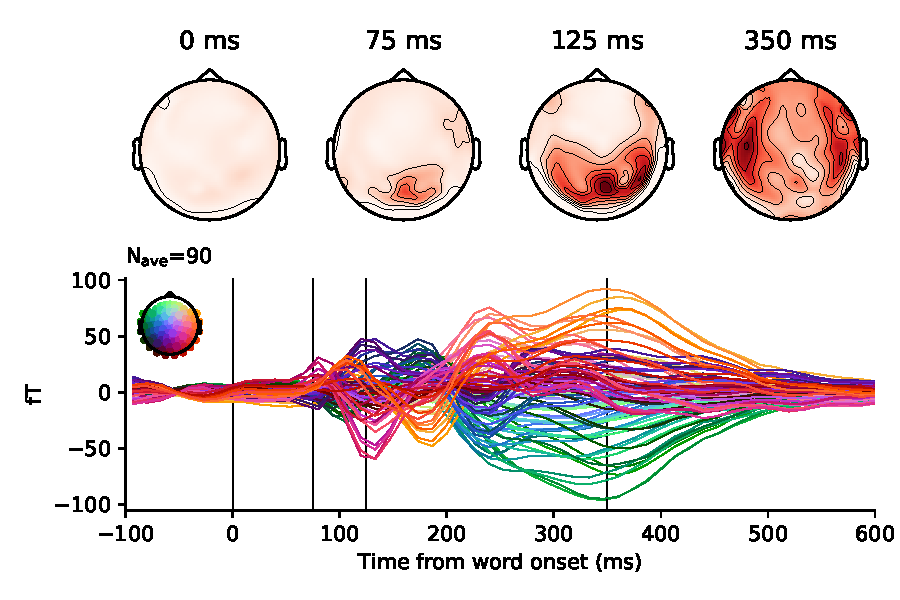
\includegraphics[width=\textwidth, trim=0cm 0cm 0cm 0cm, clip=True]{figures/meg_evoked.pdf}
  \end{minipage}\hfill
  \begin{minipage}[c]{0.4\textwidth}
    \caption{Ninety subjects read approximately 2,700 words while their brain activity was recorded with MEG. Top. Average brain response to words (word onset at t=0 ms), as viewed from above the head (red= higher gradient of magnetic flux). Bottom. Each line represents magnetometer, color-coded by spatial position. Posterior responses, typical of primary visual cortex activity, peak around 100 ms after word onset and are followed by an anterior propagation of activity typical of semantic processing in the associative cortices.
    }
    \label{fig:meg_evoked}
  \end{minipage}
\end{figure}


\subsubsection{Feature definition}

We aim to identify the word features that cause a variation in brain responses. We consider four distinct but colinear features.
%
First, 'Word Length' refers to the total number of letters. Word Length is expected to specifically cause a variation in the early evoked MEG responses (i.e. from 100 ms after stimulus onset) elicited by the retinotopically-tuned visual cortices (e.g. \citep{pegado2014timing}.).
%
Second, 'Word Frequency' indexes how frequently each word appears in Dutch and was derived with the the Zipf logarithmic scale of \citep{van2014subtlex} provided by the WordFreq package \citep{speerwordfreq}. Word Frequency is expected to specifically cause a variation in the late evoked MEG responses (i.e. from 400 ms), because it variably engages semantic processes in the temporal cortices \citep{kutas2011thirty}.
%
Third, 'Word Function' indicates whether each word is a content word (i.e. a noun, a verb, an adjective or an adverb) or a function word (i.e. a preposition, a conjunction, a determinant, a pronoun or a numeral), and was derived from Spacy's part of speech tagger \citep{spacy2}. To our knowledge, this feature has not been thouroughly investigated with MEG. Its causal contribution to reading processes in the brain thus remains unclear.
%
Finally, to verify that B2B and other methods would not inadequately identify non-causal features, we added a dummy feature, constructed from a noisy combination of Word Length and Word Frequency:
$dummy = z(length) + z(frequency) + \mathcal{N}$, where $z$ normalizes features and $\mathcal{N}$ is a random vector sampling Gaussian distribution (all terms thus have a zero-mean and a unit-variance).

This procedure yields an $X \in \mathbb{R}^{n \times d_x}$ matrix of $n\approx$ 2700 words by
$d_x=4$ features for each subject. Each of the columns of $X$ is normalized to
have a mean and a standard deviation of 0 and 1 respectively.

\subsubsection{Models and statistics}

We compare B2B to four standard methods: Forward regression, Backward regression, CCA and PLS, as implemented in scikit-learn \citep{sklearn}, and optimized with nested cross validation over twenty $l2$ regularization parameters logarithmically spaced between $10^{-4}$ and $10^4$ (for regression methods) or 1 to 4 canonical components (for cross-decomposition methods).

We used the feature importance described in Algorithm \ref{algorithm:b2b_fi} to assess the extent to which each feature $X_i$ specifically improves the prediction of held-out $Y$ data, using a 5-fold cross-validation.

Each model was implemented for each subject and each time sample independently. Pairwise comparison between models were performed using a Wilcoxon test across subjects (n=90) using the average $\Delta R$ across time.

Corresponding results are shown in Figure~\ref{fig:meg_results}.



\begin{wrapfigure}{r}{.5\textwidth}
  \vspace{-12ex}
  \begin{center}
    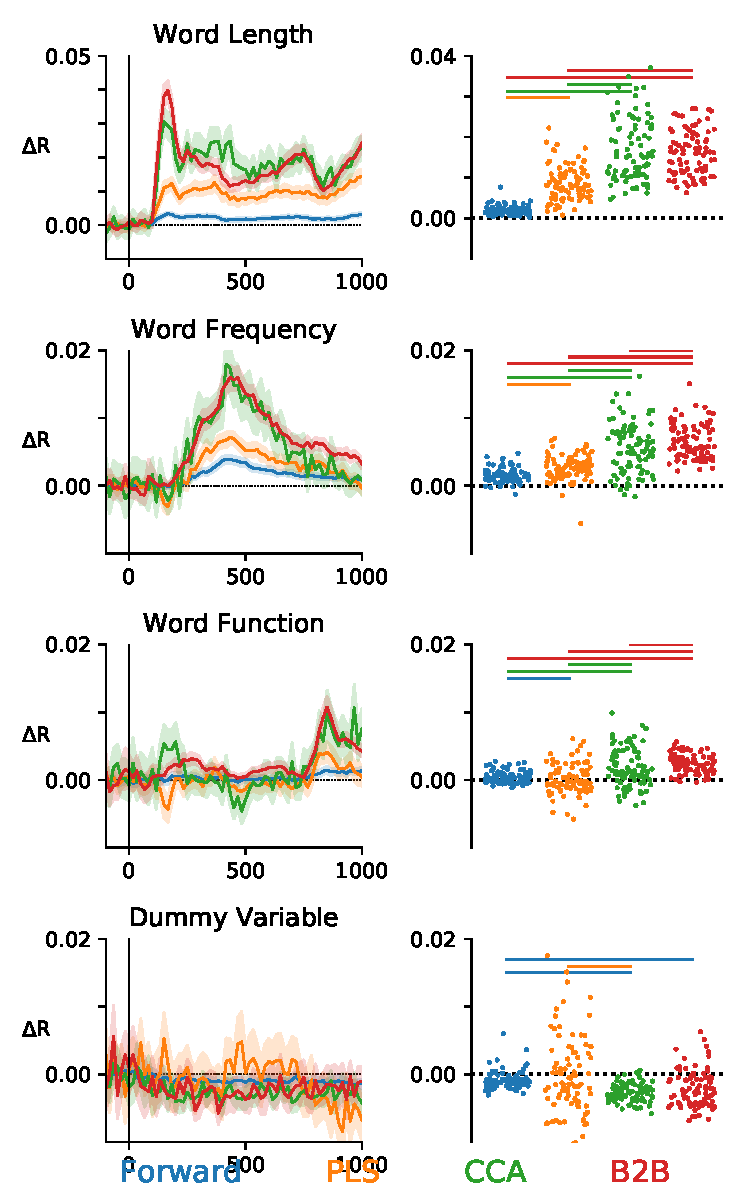
\includegraphics[width=0.48\textwidth, trim=0cm 0cm 0cm 0cm, clip=True]{figures/meg.pdf}

    \label{fig:meg_results}
  \end{center}
  \caption{Multiple models (color-coded) are compared on their ability to reliably predict single-trial MEG signals evoked by words. Left. Average improvement of correlation coefficient $\Delta R$ for each of the four features (rows). Error bars indicate standard error of the mean (SEM) across subjects. Right. Average $\Delta R$ across time for each subject (dot). Top horizontal lines indicate when B2B significantly outperforms other methods.}
  \vspace{-9ex}
\end{wrapfigure}

\subsubsection{Results}
We compared the ability of Forward regression, Backward regression, CCA, PLS and B2B to estimate the causal contribution of four distinct but collinear features on brain evoked responses to words.

Supplementary Figure \ref{fig:meg_supp} shows that the Backward model decodes the dummy variable well above chance level. In addition, the Backward model reveal a similar decoding time course for Word Length and Word Frequency, even though these features are known to specifically influence early and late MEG responses respectively \citep{kutas2011thirty}. These results illustrate that backward modelling cannot be used to estimate the causal contribution of collinear features.

We thus focus on the four remaining methods (i.e. Forward Regression, PLS, CCA, and B2B) and estimate their $\Delta R$ (i.e. the improvement of Y prediction induced by the introduction of a given feature into the model \ref{algorithm:b2b_fi}). Contrary to the Backward Model, none of the models predicted the Dummy Variable to improve the $Y$ prediction: all $\Delta R < 0$ (all $p > .089$).

Figure \ref{fig:meg_results} shows, for each model, the effects obtained across time (left) and subjects (right).

Word Length and Word Frequency improved the prediction performance of all methods: $\Delta R>0$ for all models (all $p<0.0001$). As expected, the time course associated with Word Length and Word Frequency rose from $\approx$ 100 ms and from $\approx$ 400 ms respectively. Furthermore, Word Function improved the prediction performance of all models (all $p < 0.0002$) except for PLS~($p=0.7989$). Overall, these results confirm that Word Length, Word Frequency and Word Function causally influence specific periods of brain responses to words.

To assess which model would be most sensitive to these causal discoveries, we compared B2B to other models across subjects (Figure \ref{fig:meg_results} right). For Word Length B2B outperforms all models (all $p < 0.00001$) but CCA ($p=0.0678$). For Word Frequency, B2B outperforms all models (all $p < 0.0006$). For "Word Function", B2B outperforms all models (all $p < 0.0015$). Overall, these results show that B2B reliably outperform standard methods, especially when the effects are difficult to detect.


\section{Conclusion}

\section{Acknowlegements}
Data were provided (in part) by the Donders Institute for Brain, Cognition and Behaviour.

\clearpage
\newpage

\bibliographystyle{abbrvnat}
\bibliography{paper}

\section{Appendices}

This should hold part of the tests, explanations on simulation, detailed results and stuff on meg data

\end{document}
